% mnras_template.tex
%
% LaTeX template for creating an MNRAS paper
%
% v3.0 released 14 May 2015
% (version numbers match those of mnras.cls)
%
% Copyright (C) Royal Astronomical Society 2015
% Authors:
% Keith T. Smith (Royal Astronomical Society)

% Change log
%
% v3.0 May 2015
%    Renamed to match the new package name
%    Version number matches mnras.cls
%    A few minor tweaks to wording
% v1.0 September 2013
%    Beta testing only - never publicly released
%    First version: a simple (ish) template for creating an MNRAS paper

%%%%%%%%%%%%%%%%%%%%%%%%%%%%%%%%%%%%%%%%%%%%%%%%%%
% Basic setup. Most papers should leave these options alone.
\documentclass[fleqn,usenatbib]{mnras}

% MNRAS is set in Times font. If you don't have this installed (most LaTeX
% installations will be fine) or prefer the old Computer Modern fonts, comment
% out the following line
\usepackage{newtxtext,newtxmath}
% Depending on your LaTeX fonts installation, you might get better results with one of these:
%\usepackage{mathptmx}
%\usepackage{txfonts}

% Use vector fonts, so it zooms properly in on-screen viewing software
% Don't change these lines unless you know what you are doing
\usepackage[T1]{fontenc}
\usepackage{ae,aecompl}


%%%%% AUTHORS - PLACE YOUR OWN PACKAGES HERE %%%%%

% Only include extra packages if you really need them. Common packages are:
\usepackage{graphicx} % Including figure files
\usepackage{amsmath} % Advanced maths commands
\usepackage{amssymb} % Extra maths symbols

%%%%%%%%%%%%%%%%%%%%%%%%%%%%%%%%%%%%%%%%%%%%%%%%%%

%%%%% AUTHORS - PLACE YOUR OWN COMMANDS HERE %%%%%

% Please keep new commands to a minimum, and use \newcommand not \def to avoid
% overwriting existing commands. Example:
%\newcommand{\pcm}{\,cm$^{-2}$} % per cm-squared

% Use bold font for vectors
\let\vec\mathbf

%%%%%%%%%%%%%%%%%%%%%%%%%%%%%%%%%%%%%%%%%%%%%%%%%%

%%%%%%%%%%%%%%%%%%% TITLE PAGE %%%%%%%%%%%%%%%%%%%

% Title of the paper, and the short title which is used in the headers.
% Keep the title short and informative.
\title[Hybrid multigrain]{Hybrid multigrain: A smoothed particle hydrodynamics
algorithm for small and large dust grains}

% The list of authors, and the short list which is used in the headers.
% If you need two or more lines of authors, add an extra line using \newauthor
\author[Mentiplay, Price, Laibe, \& Pinte]{%
   \parbox{\textwidth}{%
      Daniel Mentiplay$^{1}$\thanks{daniel.mentiplay@monash.edu},
      Daniel J. Price$^{1}$,
      Guillaume Laibe$^{2}$,
      Christophe Pinte$^{1,3}$}\\
   $^{1}$Monash Centre for Astrophysics (MoCA) and School of Physics and
   Astronomy, Monash University, Clayton Vic 3800, Australia \\
   $^{2}$Lyon, France \\
   $^{3}$Univ. Grenoble Alpes, CNRS, IPAG, F-38000 Grenoble, France}

% These dates will be filled out by the publisher
\date{Accepted XXX. Received YYY; in original form ZZZ}

% Enter the current year, for the copyright statements etc.
\pubyear{2020}

% Don't change these lines
\begin{document}
\label{firstpage}
\pagerange{\pageref{firstpage}--\pageref{lastpage}}
\maketitle

% Abstract of the paper
\begin{abstract}
\end{abstract}

% Select between one and six entries from the list of approved keywords.
% Don't make up new ones.
\begin{keywords}
keyword1 -- keyword2 -- keyword3
\end{keywords}

%%%%%%%%%%%%%%%%%%%%%%%%%%%%%%%%%%%%%%%%%%%%%%%%%%

%%%%%%%%%%%%%%%%% BODY OF PAPER %%%%%%%%%%%%%%%%%%

\section{Introduction}

\section{Methods}

The equations of conservation of momentum for a multiple species dust and gas
mixture are given by
%
\begin{align}
   \rho_g \frac{d \vec{v}_g}{dt} &= - \nabla P + \sum_i K_i \left(\vec{v}_{d_i}
                                    - \vec{v}_{g}\right), \\
   \rho_{d_i} \frac{d \vec{v}_{d_i}}{dt} &= - K_i \left(\vec{v}_{d_i}
                                                       - \vec{v}_{g}\right),
\end{align}
%
\\
Discuss stopping time complications for multigrain. See \citet{Hutchison:2018}.

\section{Numerical tests}

\subsection{Dusty-box}

We performed the multigrain version of the dusty-box test described in
\citet{Laibe:2011}. The dusty-box involves setting up a periodic box of uniform
density gas and dust with an initial differential velocity between the gas and
dust. In this test the equation of motion simplifies to
%
\begin{align}
   \frac{\partial \Delta \vec{V}}{\partial t} = - \Omega_n \Delta \vec{V},
\end{align}
%
where $\Delta \vec{V}$ is the differential velocity vector, and $\Omega_n$ is
the drag matrix given in Eq.~64 of \citet{Laibe:2014}. Dusty-box is a test
of the exchange of momentum between gas and dust species via the drag force. The
original dusty-box test was for a single grain size. We ran the multigrain
version described in \citet{Laibe:2014} in the linear Epstein drag regime
\citep{Epstein:1924}.

For each test we chose five dust species with grain sizes covering two orders of
magnitude---0.1 cm, 0.316 cm, 1.0 cm, 3.16 cm, and 10.0 cm---with equal mass in
each grain size bin. We performed four simulations, varying the total
dust-to-gas ratio: 0.01, 0.1, 1.0, and 10.0. The gas is initially motionless,
and each dust species has uniform velocity in the positive x-direction.

\begin{figure*}
   \begin{center}
      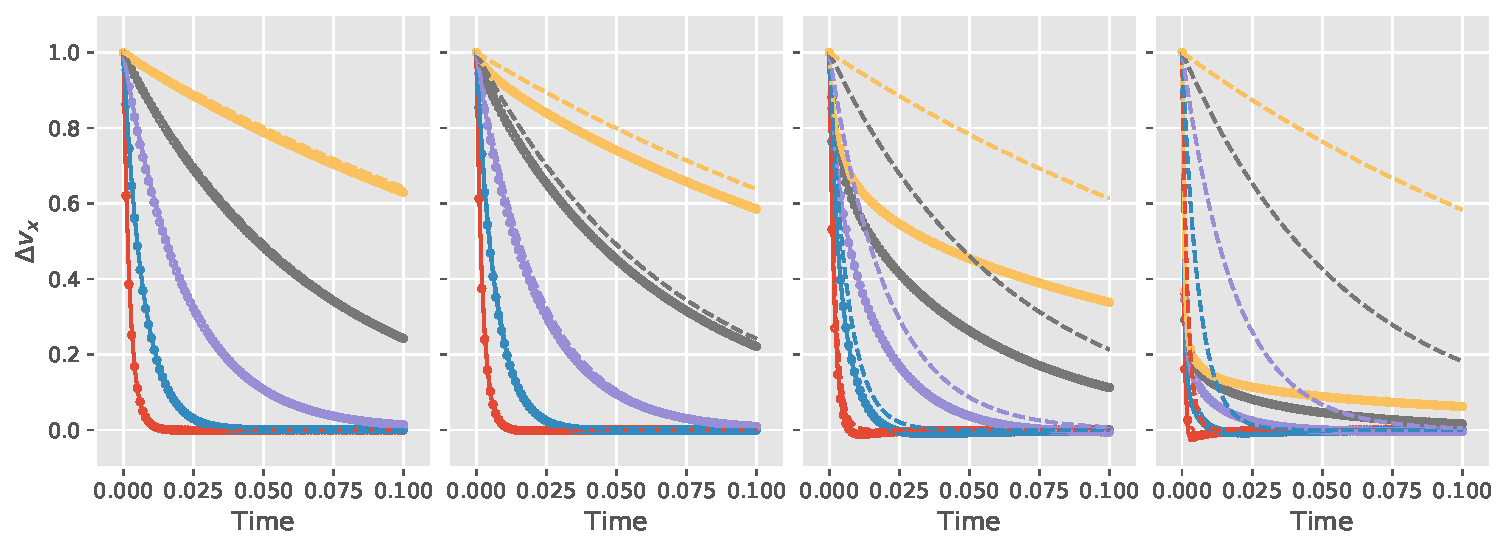
\includegraphics[width=\textwidth]{figs/delta_vx_Epstein.pdf}
      \caption{Dusty-box numerical test showing the differential velocity
         between the dust and gas. From left to right: the total dust-to-gas
         ratio is 0.01, 0.1, 1.0, and 10.0. The open circles represent the
         results from the Phantom simulation. The solid and dashed lines
         represent the analytical solution with and without, respectively,
         taking back reaction into account.\label{fig:dustybox-Epstein}}
   \end{center}
\end{figure*}

Figure~\ref{fig:dustybox-Epstein} shows the time evolution of the mean velocity
differential between the gas and each dust species, compared with analytical
solutions. The dashed lines represent the analytical solution without
backreaction from the dust on the gas. The solid lines represent the analytical
solution including backreaction. For low dust-to-gas ratio (0.01) both
analytical solutions give the same decay of differential velocity, with which
the Phantom simulation agrees. For larger dust-to-gas ratios (0.1, 1.0, and
10.0) the analytical solutions diverge, and the Phantom simulation data follows
the backreaction-inclusive solution. For dust-to-gas ratios of 1.0 and 10.0 we
see that the smallest grains (0.1 cm) slow rapidly and reverse direction with
respect to the gas before coming to the barycentric velocity.

\subsection{Dusty-wave}

Same collection of tests as dusty-box.

\subsection{Dusty-shock}
See Benitez-Llambay paper.

\section{Application}

\subsection{Circumbinary disc}

Do a comparison between multiple single grain calculations vs one multigrain
calculation focussing on dust trapping in a circumbinary disc. The figure would
show a phase difference between the dust (or gas) distribution comparing the
single-grain vs multigrain calculation.

\section{Discussion}

\section{Conclusions}

\section*{Acknowledgements}


%%%%%%%%%%%%%%%%%%%%%%%%%%%%%%%%%%%%%%%%%%%%%%%%%%

%%%%%%%%%%%%%%%%%%%% REFERENCES %%%%%%%%%%%%%%%%%%

% The best way to enter references is to use BibTeX:

\bibliographystyle{mnras}
\bibliography{multigrain-paper}


%%%%%%%%%%%%%%%%%%%%%%%%%%%%%%%%%%%%%%%%%%%%%%%%%%

%%%%%%%%%%%%%%%%% APPENDICES %%%%%%%%%%%%%%%%%%%%%

% \appendix

% \section{Some extra material}


%%%%%%%%%%%%%%%%%%%%%%%%%%%%%%%%%%%%%%%%%%%%%%%%%%


% Don't change these lines
\bsp % typesetting comment
\label{lastpage}
\end{document}
% End of mnras_template.tex
